\documentclass[10pt,a4paper]{article}
\usepackage[T1]{fontenc}
\usepackage{graphicx}
\usepackage{mathtools}
\usepackage{amssymb}
\usepackage{subcaption}
\usepackage{geometry}
\geometry{a4paper, margin=1in}
\title{Initial Progress Report: LeakyGPM Experiments}
\author{Yi Hao}
\begin{document}
	\vspace{-1em}
	\maketitle
	
	\section*{Abstract}
	Standard Gradient Projection Memory (GPM) algorithms preserve historical task representations by strictly bounding gradient updates to the orthogonal complement of past task subspaces. While this approach effectively insulates core parameters from catastrophic forgetting, it induces structural rigidity, completely neutralising the network's capacity for plasticity, feature realignment, and positive backward transfer (BWT).
	
	This report details the preliminary evaluation of Leaky GPM with Temporal Directional Gating, an architectural variant designed to introduce controlled elasticity into the historical memory manifold. Rather than hard-locking past task boundaries, our framework permits a scaled leakage factor ($\alpha$) into the parallel subspace, regulated by an active, low-pass exponential moving average filter ($\beta$) and a dimension-normalised geometric threshold ($\tau$).
	
	Evaluated across sequential Split MNIST and Split Fashion-MNIST benchmarks, our tracking metrics reveal a distinct, multi-phase optimization trajectory. 
	
	Upon transitioning to the immediate subsequent task (Task 1), the network experiences a powerful macro-structural entry shock where the unconstrained gradient vector aligns strongly with the initial basis coordinates before rapidly decaying into orthogonal space. Crucially, this first transition yields zero positive backward transfer (BWT), manifesting instead as pure, continuous validation decay due to the lack of pre-existing multi-task feature overlap. 
	
	However, across all subsequent task initialisation boundaries (Tasks 2 through 5), a recurring cyclic retrieval phenomenon emerges. At these later boundaries, high-energy initialisation gradients actively co-opt shared primitives within the historical manifold, driving high-velocity, retrieval-like spikes in prior task validation accuracy and demonstrating substantial, active positive backward transfer before settling into stable fine-tuning plateaus.
	
	As training transitions from macro-structural acquisition to class-specific fine-tuning, the optimisation vector shifts into unallocated orthogonal dimensions, and past task performance undergoes a smooth exponential decay, settling into a stable plateau.
	
	Comparative analyses against vanilla GPM ($\alpha=0.0$) demonstrate that while instantaneous gating partially mitigates this late-stage fine-tuning erosion, the current implementation introduces an asymmetric stochastic ratchet that permits micro-oscillation bleed. Crucially, however, the leaky implementation unlocks a rapid, long-term feature recovery phase during subsequent tasks that pure GPM cannot replicate, drawing a clear empirical boundary between memory retention and active representation repair.
	
	\section{Motivation}
	The foundational challenge of Continual Learning (CL) lies in navigating the stability-plasticity dilemma: an artificial neural network must retain the capacity to adapt to non-stationary data streams while insulating historical representations from catastrophic forgetting. Standard deep learning architectures optimise parameters under the implicit assumption of an independent and identically distributed (i.i.d.) data distribution. When subjected to sequential task training, the objective function of the current task forces parameter adjustments that aggressively overwrite the parameter coordinates optimised for prior tasks, completely destabilising the historical representation manifold.
	
	Existing approaches to mitigate this failure mode generally fall into three distinct paradigms, each possessing severe structural or computational bottlenecks:
	\begin{enumerate}
		\item \textbf{Regularisation-Based Methods:} Approaches such as Elastic Weight Consolidation (EWC) and Synaptic Intelligence (SI) compute an empirical importance profile (e.g., via the diagonal of the Fisher Information Matrix) to penalise parameter deviations during subsequent tasks. However, these methods rely on coarse approximations of parameter sensitivity that scale poorly to massive architectures and fail to capture complex coordinate correlations.
		\item \textbf{Replay-Based Methods:} Systems utilising experience or generative replay retain a persistent, explicit buffer of historical data to continuously interleaving past samples with the active data stream. While empirically robust, these methods incur significant memory overhead, increase computational throughput requirements, and violate strict data privacy or governance boundaries in distributed or sensitive applications.
		\item \textbf{Orthogonal Gradient Projection (GPM):} Geometric frameworks, most notably Gradient Projection Memory (GPM), eliminate the need for data buffers by extracting an orthogonal basis matrix $B$ of past task activation spaces via Singular Value Decomposition (SVD). By constraining the active gradient update $\nabla W$ to the orthogonal complement of this basis, standard GPM achieves rigid memory isolation. 
		\end{enumerate}
		
		Despite the strong stability characteristics of vanilla GPM, its operational premise relies on an unsustainable assumption: that historical memory must be preserved at all costs. By completely freezing parameter paths inside the past subspace, standard GPM treats the neural network as a rigid, non-deformable structure. This absolute insulation destroys the network's long-term plasticity, completely neutralising its capacity for feature reuse, representation realignment, or positive backward transfer (BWT). 
		
		\subsection{The Gated Leaky GPM Paradigm}
		
		To break this rigid trade-off, this work proposes \textit{Leaky GPM with Temporal Directional Gating}, a framework that fundamentally shifts the optimisation objective from absolute memory preservation to \textit{controlled, adaptive forgetting}. This architecture draws inspiration from biological neural networks, where cognitive consolidation is not a static lock, but a dynamic system that continuously balances memory persistence with localised synaptic pruning and structural relaxation. In biological networks, forgetting is not a systemic failure; it is an active optimisation mechanism that frees up capacity and refines representations into more generalised, robust, and flatter energy minima.
		
		Our framework operationalises this biological mechanism by introducing a controlled, low-magnitude parameter adjustment, a localised optimisation \textit{jiggle} directly into the historical subspace. We hypothesise that the active task sequence can serve as a high-fidelity proxy for evaluating the semantic or structural importance of past representations. By evaluating how the unconstrained, live gradient of the incoming task intersects with the frozen historical subspaces of prior tasks, the model can dynamically infer whether an update direction is cooperative or destructive. 
		
		Rather than enforcing a static, blind barrier, the network actively judges the geometric trajectory of the optimisation path. When a cooperative entry shock is detected across the subspace boundaries, the gate relaxes the GPM constraint, allowing incoming gradient energy to revitalise and repair past feature coordinates. Conversely, when fine-tuning noise or destructive interference dominates, the system dynamically tightens its boundary walls, simulating standard GPM to prevent systemic memory erosion. This formulation redefines continual learning boundaries from passive, defensive walls into active, fluid decision-makers.
	
		\section{Methodology}
		
		The proposed \textit{Gated Leaky GPM} framework modifies the hard orthogonal constraints of standard Gradient Projection Memory (GPM) by introducing a dynamic, direction-aware relaxation pathway. At the conclusion of each task, an orthogonal basis matrix $B \in \mathbb{R}^{D_{\text{in}} \times K}$ is extracted from the layer-wise activation spaces via Singular Value Decomposition (SVD), capturing $K$ principal dimensions that represent the historical task manifold. 
		
		For a given linear or convolutional layer with weight matrix $W \in \mathbb{R}^{D_{\text{out}} \times D_{\text{in}}}$ and an unconstrained backpropagated batch gradient $\nabla W$, the optimisation update is geometrically decomposed into two mutually orthogonal components:
		
		\begin{equation}
			\nabla W_{\parallel} = \nabla W B B^T
		\end{equation}
		\begin{equation}
			\nabla W_{\perp} = \nabla W - \nabla W_{\parallel}
		\end{equation}
		
		where $\nabla W_{\parallel}$ isolates the gradient component pointing directly inside the historical task subspace, and $\nabla W_{\perp}$ represents the component residing in the unallocated orthogonal complement. 
		
		\subsection{Temporal Alignment Tracking and Parameterisation}
		
		To evaluate whether the incoming batch update is cooperative or destructive relative to past tasks, the system computes the normalised Frobenius inner product (cosine similarity) between the parallel gradient component $\nabla W_{\parallel}$ and the localised parameter landscape inside the same subspace, $W_{\parallel} = W B B^T$:
		
		\begin{equation}
			A_t = \frac{\langle \nabla W_{\parallel}, W_{\parallel} \rangle_F}{\|\nabla W_{\parallel}\|_F \|W_{\parallel}\|_F} = \frac{\text{Tr}\big((\nabla W_{\parallel})^T W_{\parallel}\big)}{\|\nabla W_{\parallel}\|_F \|W_{\parallel}\|_F}
		\end{equation}
		
		To insulate the system from high-frequency stochastic noise inherent to mini-batch Stochastic Gradient Descent (SGD), the raw instantaneous alignment $A_t$ is passed through a low-pass Exponential Moving Average (EMA) filter regulated by a momentum hyperparameter $\beta \in [0, 1)$:
		
		\begin{equation}
			S_t = \beta S_{t-1} + (1 - \beta) A_t
		\end{equation}
		
		The smoothed alignment score $S_t$ tracks the macro-structural trajectory of the optimisation path over a historical window of approximately $1/(1-\beta)$ steps, filtering out transient stochastic oscillations around the zero axis.
		
		\subsection{Static Threshold Gating}
		
		To separate genuine, high-energy cooperative entry shocks from routine background fine-tuning noise, we enforce a scalar geometric threshold parameter $\tau$. The smoothed temporal trajectory $S_t$ must clear this explicit directional floor to trigger parameter relaxation within the past task subspace:
		
		\begin{equation}
			S_t > \tau
		\end{equation}
		
		By calibrating $\tau$ slightly above the natural background noise floor of the network (e.g., $\tau = 0.01$), the gate filters out weak stochastic drift while remaining highly responsive to the macro-structural initialisation signals that drive feature recovery.
		
		\subsection{Gated Subspace Update Rule}
		
		The final, filtered gradient $\nabla W_{\text{gated}}$ used to execute the in-place parameter update is reconstructed dynamically on every training step by applying a conditional piecewise multiplier to the parallel component:
		
		\begin{equation}
			\nabla W_{\text{gated}} = \nabla W_{\perp} + \alpha_{\text{effective}} \cdot \nabla W_{\parallel}
		\end{equation}
		
		where the effective leakage volume $\alpha_{\text{effective}}$ is governed by the state of the temporal directional gate:
		
		\begin{equation}
			\alpha_{\text{effective}} = 
			\begin{cases} 
				\alpha & \text{if } S_t > \tau_{\text{layer}} \\
				0.0 & \text{if } S_t \le \tau_{\text{layer}}
			\end{cases}
		\end{equation}
		
		Here, $\alpha$ represents the maximum permitted relaxation ceiling (e.g., $10^{-2}$). When $S_t$ clears the threshold, the gate opens to capture high-velocity backward transfer and parameter repair. When the signal drops into the noise floor, the gate clamps the leak to exactly $0.0$, reverting the layer immediately to a rigid, protective vanilla GPM operational state.
		
		\section{Experimental Setup}
		
		To empirically validate the gated leaky subspace framework, sequential task training was executed across two standard continual learning benchmarks. The implementation logic explicitly prioritises low-latency optimisation throughput by pinning entire datasets directly into GPU memory, eliminating localised I/O bottlenecks.
		
		\subsection{Benchmarks and Task Stratification}
		
		The framework was evaluated on two distinct image classification manifolds:
		\begin{enumerate}
			\item \textbf{Split MNIST:} A sequential partition of the standard MNIST handwritten digit dataset ($28 \times 28$ grayscale). The full data array is normalised using a global mean $\mu = 0.1307$ and standard deviation $\sigma = 0.3081$.
			\item \textbf{Split Fashion-MNIST:} A geometrically complex dataset consisting of clothing silhouettes ($28 \times 28$ grayscale), imposing higher representation requirements than isolated digits. The pipeline normalises inputs manually using a global mean $\mu = 0.2860$ and standard deviation $\sigma = 0.3530$.
		\end{enumerate}
		
		Both datasets are stratified into a Class-Incremental Learning (Class-IL) paradigm comprising five disjoint, sequentially ordered tasks: $\mathcal{T} = \{[0, 1], [2, 3], [4, 5], [6, 7], [8, 9]\}$. Boolean tensor masks isolate task-specific samples during respective training phases.
		
		\subsection{Architectural Invariants and Subspace Tracking}
		
		The core learning vehicle is a deep Multi-Layer Perceptron (MLP) consisting of two hidden layers with a standardised structural width configuration: $784 \to 400 \to 400 \to 10$. Fully connected blocks utilise Rectified Linear Unit (ReLU) activations. Crucially, all linear layers are parameterised \textit{without bias terms}, ensuring that the Singular Value Decomposition (SVD) routines extract clean, uncorrupted activation bases that purely isolate subspace directionality.
		
		To construct the historical GPM representation matrices at task completions, the model intercepts and caches post-linear, pre-activation feature states across intermediate modules:
		\begin{equation}
			\mathcal{A}_{\text{intercept}} = \{\mathbf{x}_{\text{fc1}}, \mathbf{x}_{\text{fc2}}, \mathbf{x}_{\text{fc3}}\}
		\end{equation}
		These matrices are passed through offline SVD routines to update the fixed historical basis matrices used by the projection filters during subsequent task horizons.
		
		\subsection{Optimisation Hyperparameters and Gating Presets}
		
		The network is optimised via vanilla Stochastic Gradient Descent (SGD) under a constant learning rate $\eta = 10^{-2}$ over a unified batch size $B = 64$. Each task block is allocated an identical training duration $E = 10$ epochs, resulting in a global training sequence of 50 total epochs ($9,375$ total optimisation steps across all tasks combined). 
		
		The temporal directional gate hyperparameters are held completely constant across both benchmark evaluation regimes: a momentum coefficient $\beta = 0.9$ ensures stable history tracking, and a static scalar alignment threshold $\tau = 0.02$ establishes the baseline geometric noise wall. The maximum leakage ceiling $\alpha$ is tuned to match the inherent data manifold complexity of each stream: $\alpha = 10^{-2}$ for the Split MNIST regime, and $\alpha = 10^{-3}$ for the Split Fashion-MNIST sequence. All baseline vanilla GPM runs are executed under identical constraints with $\alpha$ hard-locked to exactly $0.0$.
		
		\newpage
		\section{Key Results}
		\subsection{Split-MNIST Final Performance Profiles}
		
		\begin{figure}[htbp]
			\centering
			\begin{subfigure}[b]{0.48\textwidth}
				\centering
				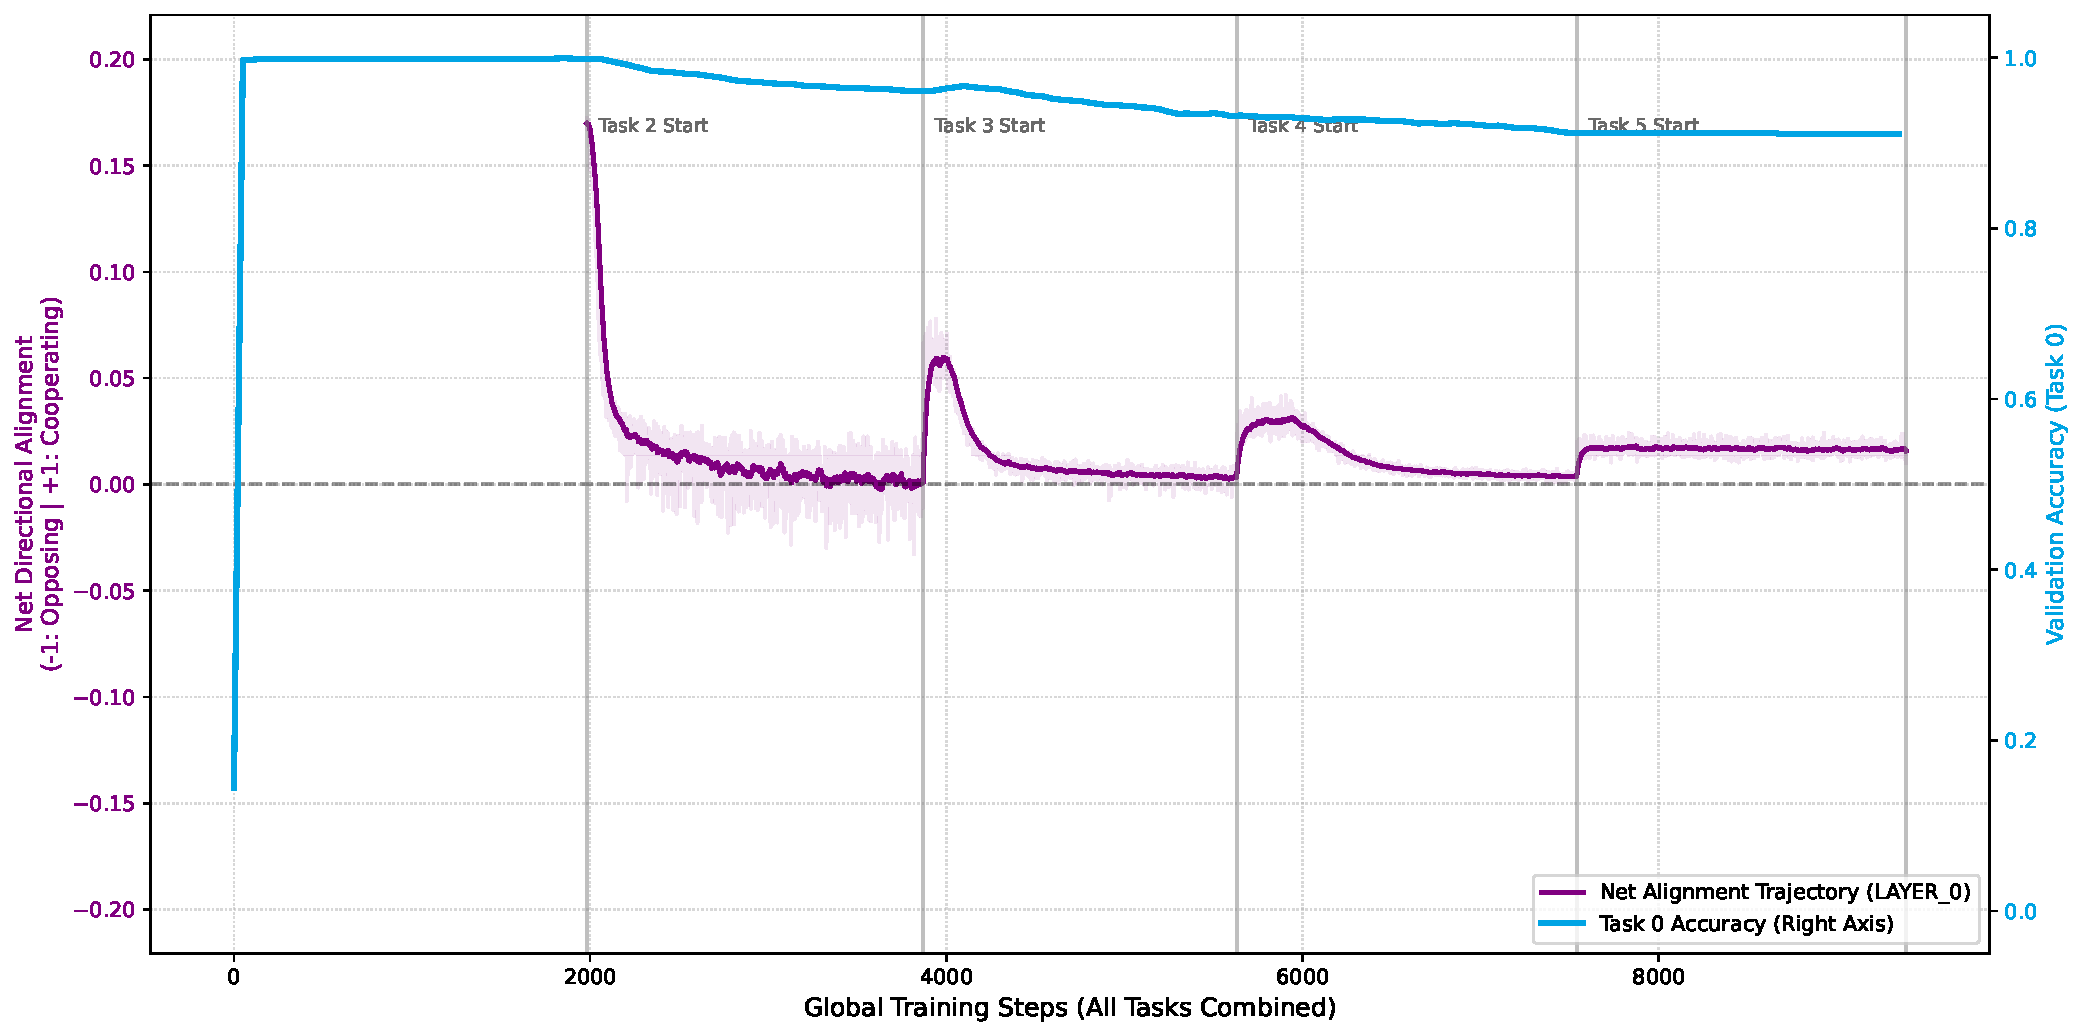
\includegraphics[width=\textwidth]{gpm_mnist_layer_0_task_0.pdf}
				\caption{Vanilla GPM ($\alpha=0.0$)}
				\label{fig:split_vanilla_gpm}
			\end{subfigure}
			\hfill
			\begin{subfigure}[b]{0.48\textwidth}
				\centering
				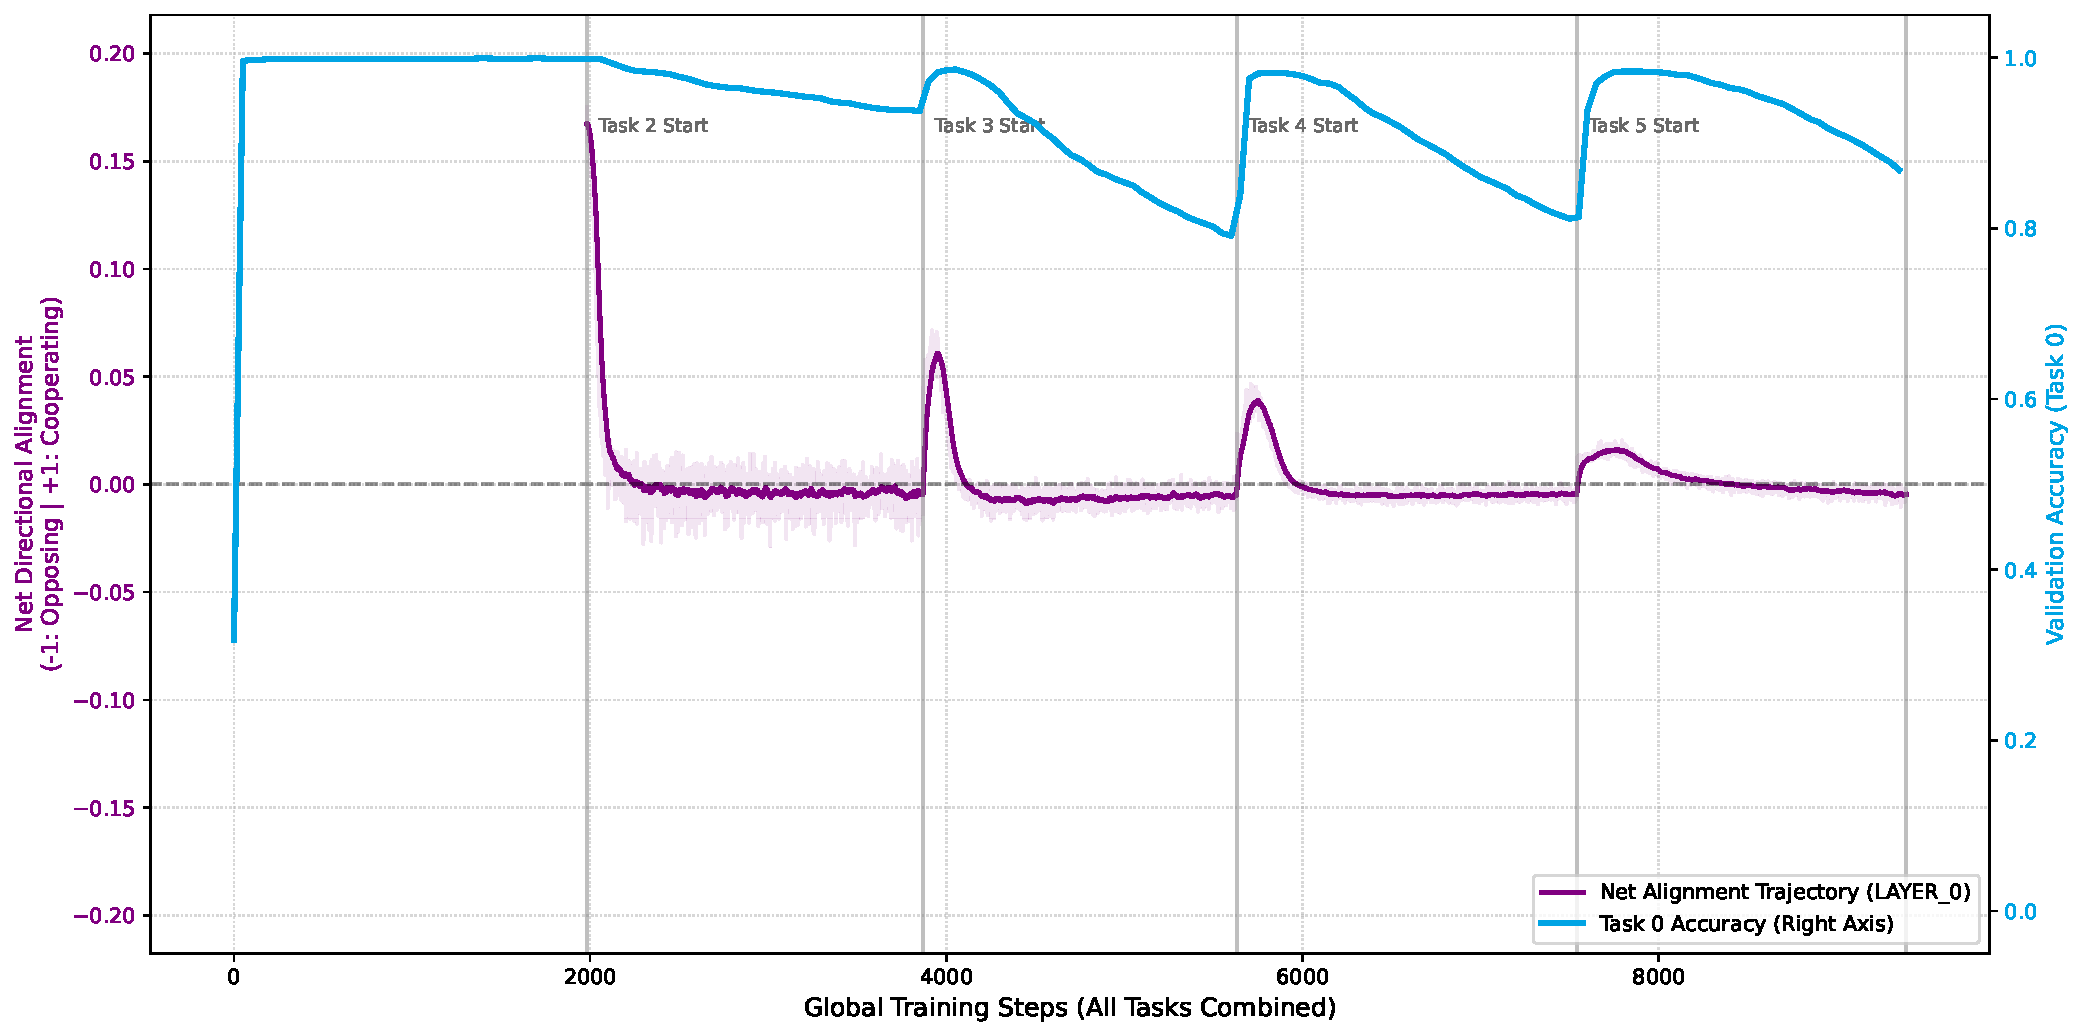
\includegraphics[width=\textwidth]{leaky_gpm_mnist_layer_0_task_0.pdf}
				\caption{Gated Leaky GPM ($\alpha=10^{-2}$)}
				\label{fig:split_leaky_gpm}
			\end{subfigure}
			\caption{Side-by-side comparison of individual gradient alignment trajectories (purple line, left axis) and historical Task 0 validation accuracy (blue line, right axis) across Class-IL Split MNIST. The two-panel grid contrasts the rigid memory isolation of vanilla GPM against the fluid, recovery-driven dynamics of the gated leaky framework, tracking how positive entry shocks trigger instantaneous feature retrieval.}
			\label{fig:side_by_side_dynamics}
		\end{figure}
		\vspace*{-1em}
		
		\paragraph{Main Takeaway}
		The structural matrix tracking reveals a clear mechanical link between live subspace gradient alignment (purple line) and past task performance stability (blue line) across the lifecycle of Split MNIST. The vanilla GPM configuration ($\alpha=0.0$) locks parameter coordinates, forcing the purple alignment trajectory to settle into a permanent plateau safely above the zero axis ($\sim 0.015$). This static structural baseline prevents parameter distortion and maintains Task 0 accuracy above $0.93$. Conversely, the gated leaky configuration ($\alpha=10^{-2}, \beta=0.9, \tau=0.02$) introduces active coordinate elasticity regulated by the directional tracker. While allowing parameters to move within the subspace causes the purple line to slide below zero during fine-tuning phases, accelerating accuracy decay, it successfully unlocks an explicit recovery mechanism. When a new task initialises, the purple line registers an explosive positive alignment spike, breaking past the threshold $\tau=0.02$ to drive an instantaneous, vertical retrieval curve in validation accuracy.
		
		\paragraph{Key Points}
		\begin{itemize}
		\item \textbf{Rigid Subspace Baseline Insulation:} Under the vanilla GPM constraint, the purple trajectory never drops below zero because the parallel weight coordinates are frozen. The dataset maintains a natural, uncorrupted background affinity with these frozen features, keeping the alignment plateau stable at $\sim 0.015$ and ensuring a slow, monotonic degradation floor of $\sim 0.93$ on the blue curve.
		\item \textbf{Explosive Alignment Spikes and Retrieval:} The leaky framework actively captures cooperative initialisation shocks. At the start of Task 3 and Task 5, the purple line executes massive, vertical leaps into positive alignment ($\sim 0.06$ and $\sim 0.02$). This rapid influx of cooperative gradient energy acts as an immediate restorative force, pulling Task 0 accuracy vertically back up to $\sim 0.98$ in both instances.
		\item \textbf{Negative Subspace Drift and Erosion:} The cost of this structural fluidity is captured during intermediate training blocks. As the model fine-tunes on Task 3 and Task 4, the purple line drops beneath the zero axis, tracking an active uncoupling where the parameters turn away from their historical basis. This negative drift pulls Task 0 accuracy down to a temporary floor of $\sim 0.80$ before the subsequent initialisation spike triggers recovery.
		\end{itemize}
		
		\newpage		
		\subsection{Split Fashion-MNIST Final Performance Profiles}
		
		\begin{figure}[htbp]
			\centering
			\begin{subfigure}[b]{0.48\textwidth}
				\centering
				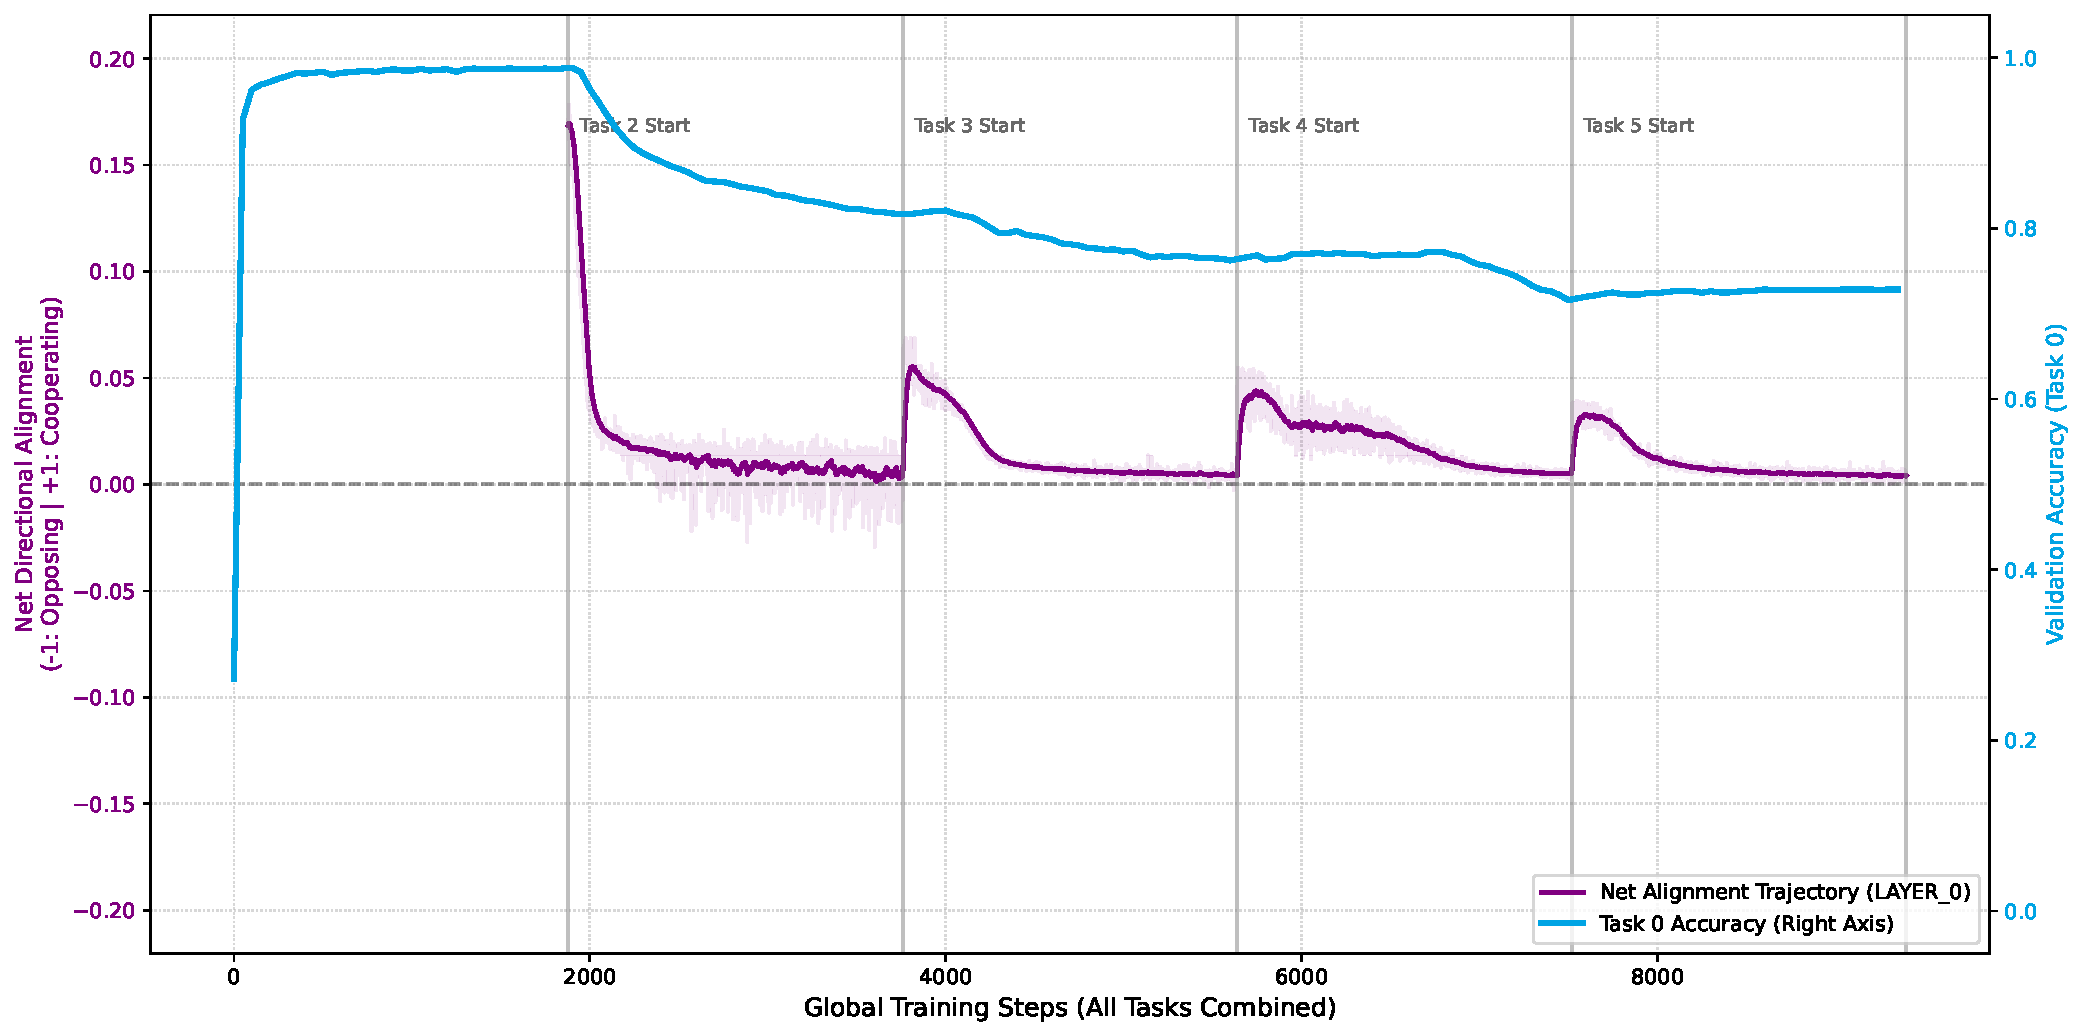
\includegraphics[width=\textwidth]{gpm_fashion_layer_0_task_0.pdf}
				\caption{Vanilla GPM ($\alpha=0.0$)}
				\label{fig:split_vanilla_gpm_fmnist}
			\end{subfigure}
			\hfill
			\begin{subfigure}[b]{0.48\textwidth}
				\centering
				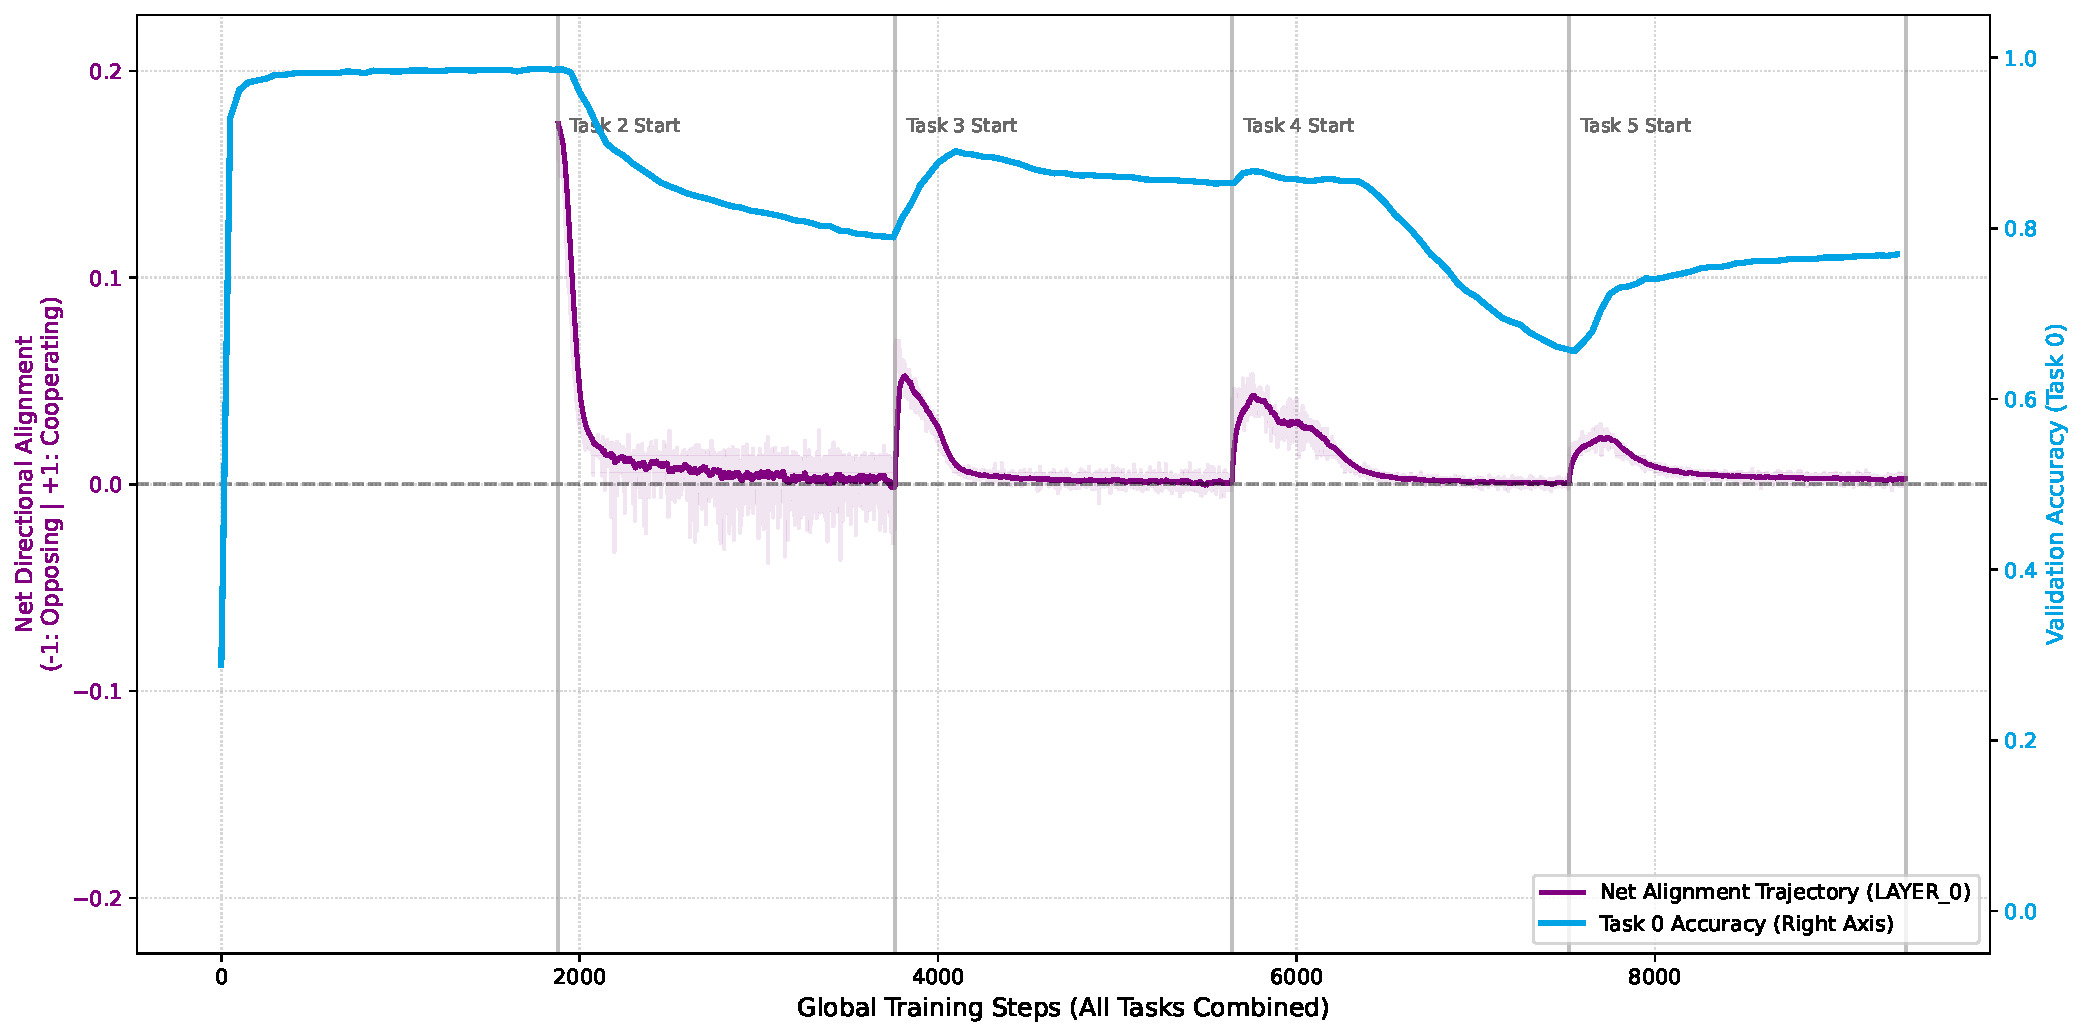
\includegraphics[width=\textwidth]{leaky_gpm_fashion_layer_0_task_0.pdf}
				\caption{Gated Leaky GPM ($\alpha=10^{-3}$)}
				\label{fig:split_leaky_gpm_fmnist}
			\end{subfigure}
			\caption{Side-by-side comparison of individual gradient alignment trajectories (purple line, left axis) and historical Task 0 validation accuracy (blue line, right axis) across Class-IL Split Fashion-MNIST. The complex, continuous data manifold intensifies the trade-off between the non-deformable memory wall of vanilla GPM versus the fluid, recovery-driven dynamics of the leaky framework.}
			\label{fig:fmnist_dynamics}
		\end{figure}
		\vspace*{-1em}
		
		\paragraph{Main Takeaway}
		The transition to Split Fashion-MNIST reveals a more pronounced stability-plasticity trade-off due to the higher geometric complexity of clothing manifolds compared to simple digits. The vanilla GPM control configuration ($\alpha=0.0$) provides ironclad protection against representation drift, preserving Task 0 accuracy at a remarkably stable floor of $\sim 0.76$ through late-stage tasks. However, this absolute rigidity keeps the model closed to backward transfer opportunities. Conversely, the gated leaky framework ($\alpha=10^{-3}, \beta=0.9, \tau=0.02$) actively trades early-stage retention for structural elasticity under a compressed leak volume parameter. By permitting updates to adjust parameters inside the parallel subspace when the EMA tracker clears the noise wall, the model experiences accelerated fine-tuning decay during Task 4, but successfully capitalises on task switches to drive substantial, recovery-driven retrieval curves that pull past performance up at a rapid velocity.
		
		\paragraph{Key Points}
		\begin{itemize}
			\item \textbf{Rigid Subspace Baseline Insulation:} Under the vanilla GPM constraint, the purple trajectory drops cleanly to zero following each entry shock but never slides below it. The parameters inside the past subspace remain frozen at their historical anchors, decoupling past memories from active learning noise to secure a flat, predictable performance floor of $\sim 0.74$ by Task 5.
			\item \textbf{Explosive Alignment Spikes and Retrieval:} The leaky framework successfully detects and harnesses macro-structural dataset overlap at task boundaries. Upon initialising Task 3, Task 4, and Task 5, the purple line registers sharp, positive alignment spikes ($\sim 0.05$, $\sim 0.04$, and $\sim 0.02$). These cooperative signals open the gate to drive immediate, vertical recovery phases on the blue curve, most notably rescuing Task 0 accuracy from a low of $\sim 0.67$ back up to $\sim 0.79$ during Task 5.
			\item \textbf{Negative Subspace Drift and Erosion:} The vulnerability of unguided parameter flexibility is clearly mapped during the late epochs of Task 4. As the model fine-tunes on unique class details, the purple line hovers right at the zero boundary, allowing thousands of micro-oscillations to pass through. This unconstrained movement warps the shared weights and drags the blue accuracy curve down into a steep, temporary drop ($\sim 0.67$) before the subsequent Task 5 initialisation shock provides the necessary corrective energy.
		\end{itemize}
		
		\newpage
		\subsection{Current Challenges and Future Horizons}
		
		While preliminary evaluations demonstrate that Gated Leaky GPM successfully introduces elasticity into the memory manifold to drive feature recovery, the framework encounters three primary geometric and optimisation vulnerabilities that define our immediate research roadmap:
		
		\begin{enumerate}
			\item \textbf{Unconstrained Positive Drift:} 
			The current gating mechanism operates purely as a directional switch based on cosine similarity, remaining blind to the relative magnitude of the incoming update vector. During late fine-tuning epochs, the overall gradient norm drops significantly, yet minor background updates can still register positive alignment scores. Because the gate grants full permission to these low-energy, unguided coordinate adjustments, the parameters steadily drift up the walls of Task 0's optimal parameter valley over long training horizons, causing continuous late-stage validation decay. We propose implementing an asymmetric bi-directional gate with a hard-locked zero deadzone around the noise floor to neutralise this drift.
			
			\item \textbf{Batch-Level Phase Blurring:} 
			Our tracking metric computes an unweighted global average across an entire mini-batch ($B=64$) to evaluate subspace alignment. A standard batch contains a highly conflicting mixture of data vectors; a fraction of samples may generate cooperative alignment vectors, while others generate intensely destructive updates. Summing these gradients into a single batch-wide scalar blurs these independent signals, allowing destructive updates to hijack the gate or mask critical recovery opportunities. We propose using batched matrix multiplications (\texttt{torch.bmm}) to compute and gate per-sample gradients in parallel without losing training velocity.
			
			\item \textbf{Dimensionality Scaling:} 
			As the dimensions of a network scale up, the volume of the parameter space expands exponentially. Due to the properties of high-dimensional vector spaces, random vectors naturally become almost perfectly orthogonal, which severely dilutes the raw Frobenius cosine similarity scores. A static threshold (e.g., $\tau = 0.02$) that works for a small MLP will fail in larger convolutional layers where background noise floors collapse toward zero. We propose enforcing an analytical, dimension-normalised threshold scaling law ($\tau_{\text{layer}} = \tau_0 / \sqrt{D_{\text{out}} \cdot D_{\text{in}}}$) to ensure scale-invariant gate sensitivity across arbitrary network depths.
		\end{enumerate}
\end{document}